In 1982, a new neutral-beam injection heating system was install in the ASDEX tokamak, which pushed it into a new realm.
A new level of energy confinement time was achieved, measured to be a factor of 2 or more than previous.
This state of operation was coined the high-confinement (H-) mode, and is now considered necessary for the future of nuclear fusion as an energy source \cite{arnoux_how_2009} \cite{wagner_development_1984}.
With this new level of energy confinement, the community got one step closer toeconomic fusion power plants.
The details of this transition, however, are not fully understood.

\section{Characteristics of L- and H-Mode}
Transport of particles and energy in tokamaks has been discovered to be significantly dominated by anomalous (turbulent) transport, which is generally assumed to be generated by turbulence, driven by micro-instabilities.
Low-confinement mode, L-mode, is dominated by this transport at the edge.
The formation of H-mode is due to the suppression of this turbulent transport at the edge of the plasma; thus is catagorized as a transport barrier.
The plasma edge is defined to be the thin boundary layer of the plasma just inside the separatrix.

\begin{figure}[b]
\begin{minipage}{0.48\linewidth}
	\centering
	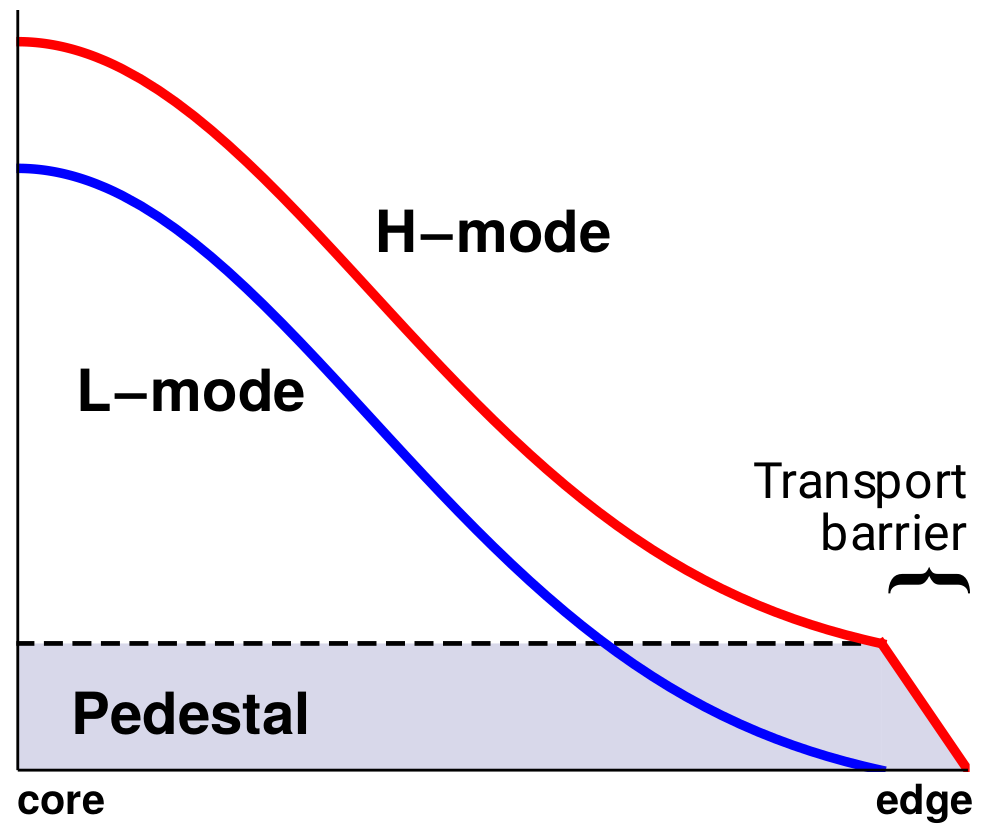
\includegraphics[width=0.8\textwidth]{../Graphics/L-mode_H-mode_compare.png}
\end{minipage}
\hfill
\begin{minipage}{0.48\linewidth}
	\caption{A comparison of the radial pressure profiles of L-mode and H-mode.
	The profile of H-mode can be thought of as on a `pedestal,' in which the pressure profile is increase in the core.
	This is due to the transport barrier that is formed at the edge \cite{weymiens_bifurcation_2014}.}
	\label{fig:L-mode_H-mode_compare}
\end{minipage}
\end{figure}

H-mode is characterized by its pressure profile significantly raised compared to that of L-mode, and is said to sit on a `pedestal.'
Accordingly, there is a steep gradient in the pressure at the edge of the plasma, shown and compared to L-mode in Figure~\ref{fig:L-mode_H-mode_compare} \cite{weymiens_bifurcation_2014}.
This results in an increase temperature in the core.

\section{H-mode Mechanism and Transition}
The prevailing hypothesis for the overarching mechanism for H-mode is that high auxiliary power developes strong sheared plasma flow and suppresses transport \cite{freidberg_plasma_2007}.
The shear stress dissociates smaller turbulent structions, with their energy and momenta transferred to larger flows \cite{staps_backstepping_2017}.
FIX!! The $\mathbf{E}\times\mathbf{B}$-velocity shear, which has been modeled many times.

